%%% fs-seim-intro - Introduction

\label {fs-intro}

Nowadays, a lot of real-life applications use stream processing for network monitoring, financial analytics, training machine learning models, etc. State-of-the-art industrial stream processing systems, such as Flink \cite{carbone2015apache}, Samza \cite{Noghabi:2017:SSS:3137765.3137770}, Storm \cite{apache:storm}, Heron \cite{Kulkarni:2015:THS:2723372.2742788}, are able to provide low-latency and high-throughput in distributed environment for this kind of problems. However, providers of the order-sensitive computations still remain suboptimal. Most of these systems assume that events are fed to the system with monotonically increasing timestamps or with minor inversions. Often, such timestamps can be assigned at system's entry. Nevertheless, even if input items arrive monotonically, they can be reordered because of the subsequent parallel and asynchronous processing. In this case, order-sensitive operations located deeper in data flow pipeline can be broken. Figure ~\ref{break-order-dataflow} shows the example of common distributed stream processing pipeline that breaks the input order of the operation 2, even if input is monotonic and links between operations guarantee FIFO order.

\begin{figure}[htbp]
  \centering
  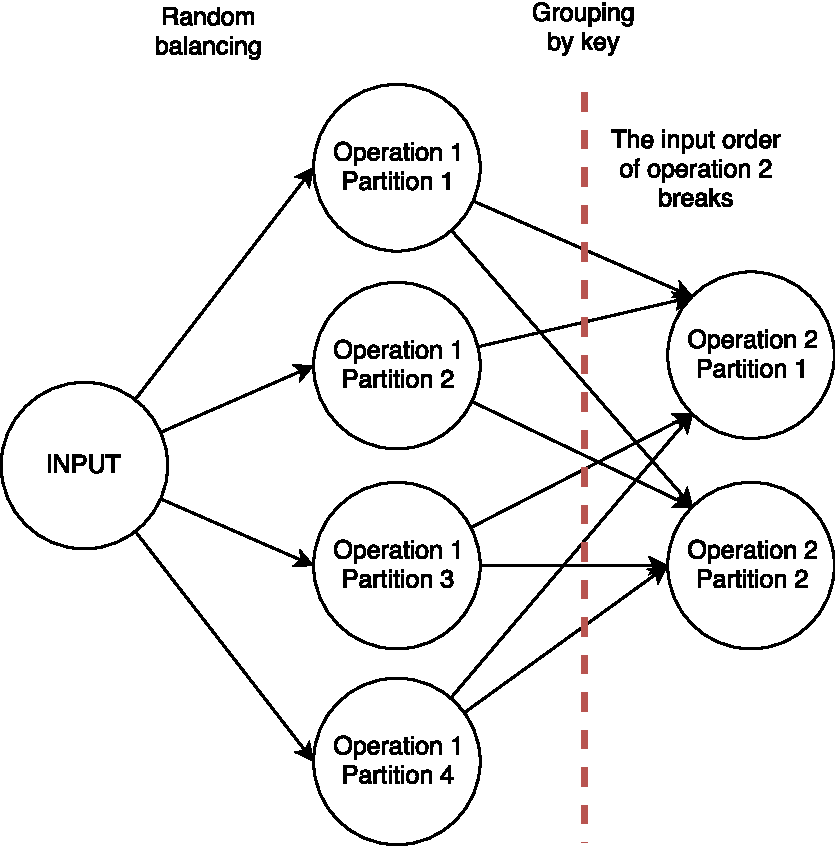
\includegraphics[width=0.38\textwidth]{pics/break_order_pipeline}
  \caption{An  example of common distributed stream processing pipeline that breaks the input order of operation}
  \label {break-order-dataflow}
\end{figure}

The typical way to achieve in-order processing is to set up a special buffer in front of operation. This buffer collects all input items until some user-provided condition is satisfied. Then the contents of the buffer is sorted and fed to the operation. The main disadvantage of such technique is latency growth. This issue becomes even more significant if the processing pipeline contains several operations that require ordered input. 

The alternative is to develop business logic tolerant to out-of-order items. However, this approach  is suitable only for a limited set of tasks. Moreover, it may dramatically complicate the business-logic, which can lead to the maintenance cost increase and is error-prone.

In this paper we introduce an optimistic approach to handle out-of-order items. Our evaluation demonstrates its advantages compared to existing solutions. The contributions of this paper are the following: 

\begin {itemize}
  \item Definition of new optimistic technique to handle out-of-order items in stateful operations
  \item Analysis of properties of this approach
  \item Demonstration of working example that applies proposed method
\end {itemize}

The rest of the paper is structured as follows: in section~\ref{fs-stream} we formalize the preliminaries of stream processing, the examples of tasks that require ordered input are described in section~\ref{fs-tasks}, the typical approaches for handling out-of-order events are discussed in~\ref{fs-typical}, our optimistic technique is detailed in~\ref{fs-optimistic} and its performance is demonstrated in ~\ref{fs-experiments}, the main differences between proposed method and existing ones are shown in~\ref{fs-related}, finally we discuss the results and our plans in~\ref{fs-conclusion}.
